%\documentclass{article}
%\documentclass[journal]{IEEEtran}
\documentclass[letterpaper, twoside, openright]{report}
%\documentclass{ActaOulu}
%\documentclass{memoir}

\usepackage{color}
\usepackage{graphicx}
\usepackage{authblk}
\usepackage{mathtools}

\usepackage{url}
\usepackage{hyperref}
\hypersetup{colorlinks=true, filecolor=blue, citecolor=red, linkcolor=black, urlcolor=blue}

\begin{document}

\title{Ultrasonics Spectrometer Code Manual}
\author{Matthew Rothfuss\thanks{\href{mailto:mrengr@phys.ksu.edu}{mrengr@phys.ksu.edu}, \href{mailto:mrengr@k-state.edu}{mrengr@k-state.edu}, \href{mailto:rothfuss212@gmail.com}{rothfuss212@gmail.com}}}
\affil{Department of Animal Science and Food Industry, Kansas State University}

\maketitle

%\begin{figure}[h]
%    \centering
%    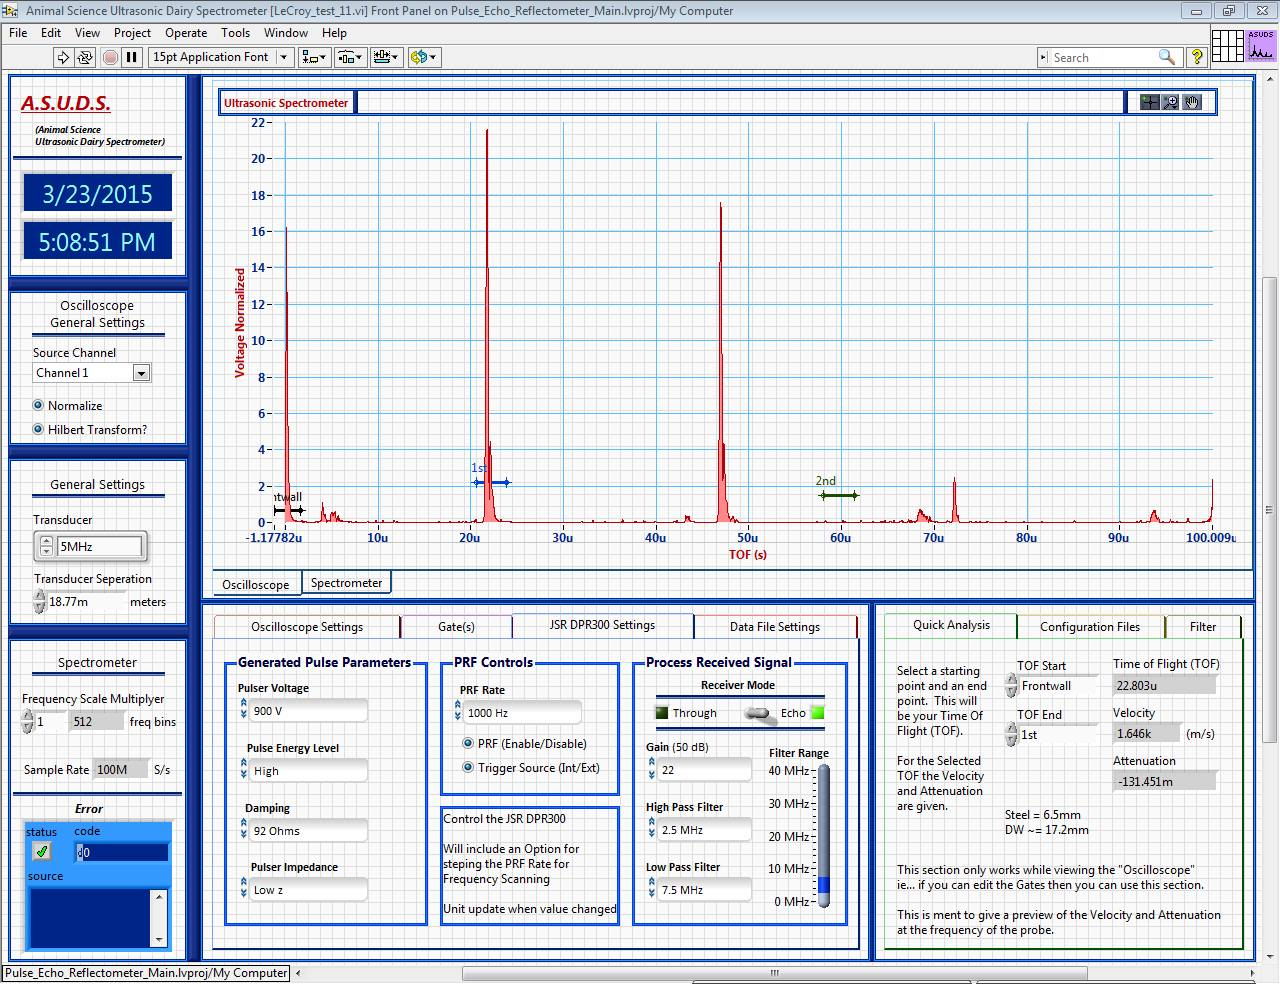
\includegraphics[width=3.0in]{title_page}
%    \caption{Animal Science Ultrasonic Dairy Spectrometer (ASUDS)}
%    \label{Title_Pic}
%\end{figure}

%\begin{abstract}
%Start with an area of civil society where deliberation is occurring (or needs to occur). Identify the barriers to more effective deliberation that are present in this situation and explain them using concepts found in this week's readings. Is there a way for argument/advocacy/debate to address this issue? DO NOT use an example already found in the text or extensively discussed in class---there are plenty of other ones out there for you to choose from.
%\end{abstract}


\tableofcontents


\chapter{LabView Basics}

\section{Introduction}

LabVIEW	(short	for	\textbf{Lab}oratory	\textbf{V}irtual	\textbf{I}nstrumentation	\textbf{E}ngineering	\textbf{W}orkbench) is a development environment for visual programming, developed by National Instruments (\href{http://www.ni.com/}{www.ni.com}). The code files (or program files) are identified by the \textbf{.vi} extension called \textbf{Virtual Instruments} or \textbf{VIs} for short. This graphical language is most commonly used for data acquisition, instrument control, signal processing (analysis), industrial automation, and more.

The next section will cover some basics of LabVIEW design and operation. For additional resources, the current (2013) LabVIEW Getting Started Manual is located \href{http://www.ni.com/pdf/manuals/373427j.pdf}{here}.

\subsection{Additional Resources}

\cite{gomez_alvarez-arenas_air-coupled_2003}

\subsection{Advocate the Issue}

 

\section{Conclusion}



\bibliography{ultrasound-ref-01}
\bibliographystyle{unsrt}

\end{document}
